\documentclass[conference]{IEEEtran}
\usepackage{cite}
\usepackage{amsmath,amssymb,amsfonts}
\usepackage{algorithmic}
\usepackage{graphicx}
\usepackage{textcomp}
\usepackage{xcolor}
\usepackage{kotex}
\usepackage{float}
\def\BibTeX{{\rm B\kern-.05em{\sc i\kern-.025em b}\kern-.08em
    T\kern-.1667em\lower.7ex\hbox{E}\kern-.125emX}}
\begin{document}

\title{Nanuda: A Group Expenses Manager}

\author{\IEEEauthorblockN{1\textsuperscript{st} Abia Herlianto}
\IEEEauthorblockA{\textit{School of Computer Science} \\
\textit{BINUS University}\\
\textit{Team MONEY}\\
Jakarta, Indonesia \\
abiaph@live.com}
\and
\IEEEauthorblockN{2\textsuperscript{nd} Hugo Ravé}
\IEEEauthorblockA{\textit{General Engineering} \\
\textit{ESILV PARIS-LA DEFENSE}\\
\textit{Team MONEY}\\
Paris, France \\
hugorave07@gmail.com}
\and
\IEEEauthorblockN{3\textsuperscript{rd} Nadya Hartanto}
\IEEEauthorblockA{\textit{School of Information Systems} \\
\textit{BINUS University}\\
\textit{Team MONEY}\\
Jakarta, Indonesia \\
ndhartanto1@gmail.com}
}

\maketitle

\begin{abstract}
Users create a "group" composed of several people. Users then invite these people to the group. Users add expenses and split the costs with either all, some, or no members of the group. Users can add descriptions for each expense. Users can also customise how the costs are split. Users can see a summary of how much they owe to others and how much others owe to others. The summary of how much users owe changes as users spend and pay.
\end{abstract}

\begin{IEEEkeywords}
expenses, finance, management
\end{IEEEkeywords}

\begin{table}[htbp]
\caption{Role Assignments}
\label{tab:role-assignments}
\begin{tabular}{|c|c|c|}
\hline
\textbf{Role} & \textbf{Name} & \textbf{Task Description} \\ \hline
User/Customer &
  \begin{tabular}[c]{@{}c@{}}Nadya\\ Hartanto\end{tabular} &
  \begin{tabular}[c]{@{}c@{}}Tests the application for bugs and\\ issues. Provides feedback to the\\ Development Manager. Also provides\\ feedback on UX and UI quality.\end{tabular} \\ \hline
\begin{tabular}[c]{@{}c@{}}Software\\ Developer\end{tabular} &
  \begin{tabular}[c]{@{}c@{}}Abia Putrama\\ Herlianto\end{tabular} &
  \begin{tabular}[c]{@{}c@{}}Implements software based on design.\\ Fixes bugs and issues.\end{tabular} \\ \hline
\begin{tabular}[c]{@{}c@{}}Development\\ Manager\end{tabular} &
  Hugo Ravé &
  \begin{tabular}[c]{@{}c@{}}Designs software based on\\ requirements and feedback from\\ User/Customer. Organises,\\ schedules, and manages development.\end{tabular} \\ \hline
\end{tabular}
\end{table}

\section{Introduction}
When there are shared expenses in a group, it can be complicated to split the costs and gather the money that each person should pay. The usual solution is to have one or several individuals cover the cost of the entire group, and from there the remaining group members would pay their share to those who covered the cost.

The problem that arises from this is keeping track of these expenses. This is especially true for groups that meet regularly; for example, a group of friends going on a trip. Keeping track of who covered what for how much and who owes whom how much can quickly get out of hand. The solution that we propose is a simple application where these expenses can be organised, viewed, and accessed by all members of a certain group.

The name Nanuda comes from Korean 나누다, meaning 'to divide (up), to split (up)'. The name was chosen because our own experiences in splitting expenses in Korea was the reason we thought up of the idea.

There are several existing applications that perform a similar function, with different individual features. These include Tricount and Sesterce.
\section{Requirements}

\begin{enumerate}
    \item This application should run on the Android operating system.
    \item \textbf{Groups}
        \begin{enumerate}
            \item The application should display existing, joined groups.
            \item The user should be able to open the groups.
            \item The user should be able to create new groups and join existing groups.
            \item The user should be able to join a group using a simple link.
            \item The user should be able to edit and delete existing joined groups.
            \item The user should be able to save changes to and sync with the groups data in the server.
            \item By default, the application should display a sample group.
            \item A group should have one or more participants.
            \item A group should use only one currency out of several options.
        \end{enumerate}
    \item \textbf{Expenses}
        \begin{enumerate}
            \item The application should display existing expenses in the group.
            \item The user should be able to open the expenses.
            \item The user should be able to create new expenses in the group.
            \item The user should be able to edit and delete existing expenses.
            \item The user should be able to save changes to and sync with the group expenses data in the server.
            \item The user should be able to determine who pays and who owes.
            \item The user should be able to determine how much each participant owes.
        \end{enumerate}
    \item \textbf{Balances}
        \begin{enumerate}
            \item The application should display how much each participant currently owes or is owed in total.
            \item If participants owe to each other, the application should show how to settle the owed amounts.
        \end{enumerate}
\end{enumerate}

\section{Development Environment}
\subsection{Choice of Software Development Platform}
\begin{enumerate}
    \item \textbf{Platform}
        \newline
        \begin{figure}[htbp]
            \centerline{
\includegraphics[width=50mm,scale=0.5]{img/logo-android.png}}
            \caption{Android}
            \label{fig:android-logo}
        \end{figure}
        \newline
        For Nanuda, we have chosen the \textbf{Android} mobile operating system as the platform for several reasons:
        \begin{enumerate}
            \item Nanuda needs to be on a mobile platform for quick access and easy use
            \item Android is the best-selling mobile OS worldwide
            \item Resources for development on Android are widely available and at no cost
        \end{enumerate}
        
    \item \textbf{Programming Language}
        \newline
        \begin{figure}[htbp]
            \centerline{
\includegraphics[height=25mm,scale=0.5]{img/logo-java.png}}
            \caption{Java}
            \label{fig:java-logo}
        \end{figure}
        \newline
        For the development of Nanuda, we use the \textbf{Java} programming language. Java is a class-based, object-oriented programming language and one of the world's most popular and widely used programming languages. We chose to use Java for two reasons:
        \begin{enumerate}
            \item Java is the language used to develop Android apps through the Android SDK
            \item We are familiar with Java and have used it in the past
        \end{enumerate}
    \item \textbf{Cost Estimation}
        \newline
        For the development of Nanuda, all of the resources used are either free of charge or have both free and paid options. For the resources with free and paid options, we have decided to use the free option. As such, the development of Nanuda requires no cost.
        \begin{center}
            \begin{table}[H]
            \centering
            \caption{Cost Estimation}
            \label{tab:cost-estimation}
            \begin{tabular}{|p{6em}|p{10em}|p{4em}|}
                \hline
                \textbf{Resource} & \textbf{Role Description} & \textbf{Cost} \\
                \hline
                Android Studio & Android Development IDE & 0 \\
                \hline
                Back4App & Backend Server & 0 \\
                \hline
                Overleaf & Online, Collaborative LaTeX Writing Tool & 0 \\
                \hline
                GitHub & Remote Repository and Version Control System & 0 \\
                \hline
                GitHub Desktop & GUI for GitHub & 0 \\
                \hline
                MockFlow & UI Planning Platform & 0 \\
                \hline
            \end{tabular}
            \end{table}
        \end{center} 
        
    \item \textbf{Development Environment} 
    \begin{itemize}
        \item \textbf{Android Studio Version 4.1} 
        \begin{figure}[htbp]
            \centerline{
\includegraphics[width=50mm,scale=0.5]{img/logo/logo-android-studio.png}}
            \caption{Android Studio}
            \label{fig:androids-studio-logo}
        \end{figure}
        \newline
        Android Studio was chosen because it is the official IDE for the Android operating system.
        \newline
        \item \textbf{Back4App} 
        \begin{figure}[htbp]
            \centerline{
\includegraphics[width=50mm,scale=0.5]{img/logo/logo-Back4app.png}}
            \caption{Back4App}
            \label{fig:back4app-logo}
        \end{figure}
        \newline
        Back4App is a low-code backend based on the open-source Parse Platform. Back4App was chosen due to its accessibility and ease of use, allowing anyone to make apps faster without managing infrastructure. It can easily be integrated on any mobile or web app through GraphQL, Rest APIs, or the various Parse SDKs.
        \newline
        \item \textbf{Overleaf} 
        \begin{figure}[H]
            \centerline{
\includegraphics[width=50mm,scale=0.5]{img/logo/logo-overleaf.png}}
            \caption{Overleaf}
            \label{overleaf-logo}
        \end{figure}
        Overleaf was chosen because of its popularity and the effectiveness of its features, namely simple, in-browser editing, immediate compilation, easy sharing and collaborative editing.
        \newline
        \item \textbf{GitHub} 
        \begin{figure}[H]
            \centerline{
\includegraphics[width=50mm,scale=0.5]{img/logo/logo-github.png}}
            \caption{GitHub}
            \label{github-logo}
        \end{figure}
        GitHub was chosen for Nanuda's remote repository because of our familiarity with it in comparison to other version control systems.
        \newline
        \item \textbf{GitHub for Desktop}
        \begin{figure}[H]
            \centerline{
\includegraphics[width=50mm,scale=0.5]{img/logo/logo-githubdesktop.png}}
            \caption{GitHub for Desktop}
            \label{githubdesktop-logo}
        \end{figure}
        GitHub for Desktop was chosen instead of the regular, CLI-based system to interact with GitHub because of its simplicity and intuitiveness.
        \newline
        \item \textbf{MockFlow} 
        \begin{figure}[H]
            \centerline{
\includegraphics[width=50mm,scale=0.5]{img/logo/logo-mockflow.jpg}}
            \caption{MockFlow}
            \label{mockflow-logo}
        \end{figure}
        MockFlow is a powerful online UI planning platform. MockFlow was chosen due to its rich pre-made library of components as well as its powerful editor, even in its free package.
    \end{itemize}
\end{enumerate}

\subsection{Software in use}
\begin{enumerate}
    \item \textbf{Tricount} \\
        \begin{figure}[htbp]
            \centerline{
\includegraphics[width=50mm,scale=0.5]{img/logo-tricount.png}}
            \caption{Tricount}
            \label{fig:tricount-logo}
        \end{figure}
        \begin{itemize}
            \item \textbf{Rating}: 4.8 stars (48,000 ratings) on Google Play Store
            \item \textbf{Downloads}: 1 million+ on Google Play Store
            \item \textbf{Features}:
                \begin{itemize}
                    \item Optional log in feature allows all a user's Tricounts to be linked to a user's profile
                    \item Share simple link so other users can join groups and see expenses
                    \item Anyone in a group can add their own expenses
                    \item Splitting expenses unevenly
                    \item Works offline
                    \item Works on both the web and mobile (Android, iOS, and Windows Phone)
                    \item Optional push notifications when someone edits or adds expenses
                    \item Sort expenses by categories
                    \item Several other paid features such as statistics
                \end{itemize}
            \item \textbf{Differences}:
                \begin{itemize}
                    \item Nanuda does not have log in feature to be as lightweight as possible
                    \item Only mobile app
                    \item No push notifications
                    \item No expense categories
                    \item Does not have some of Tricount's paid features such as statistics
                \end{itemize}
        \end{itemize}
    \item\textbf{Sesterce} \\
        \begin{figure}[htbp]
            \centerline{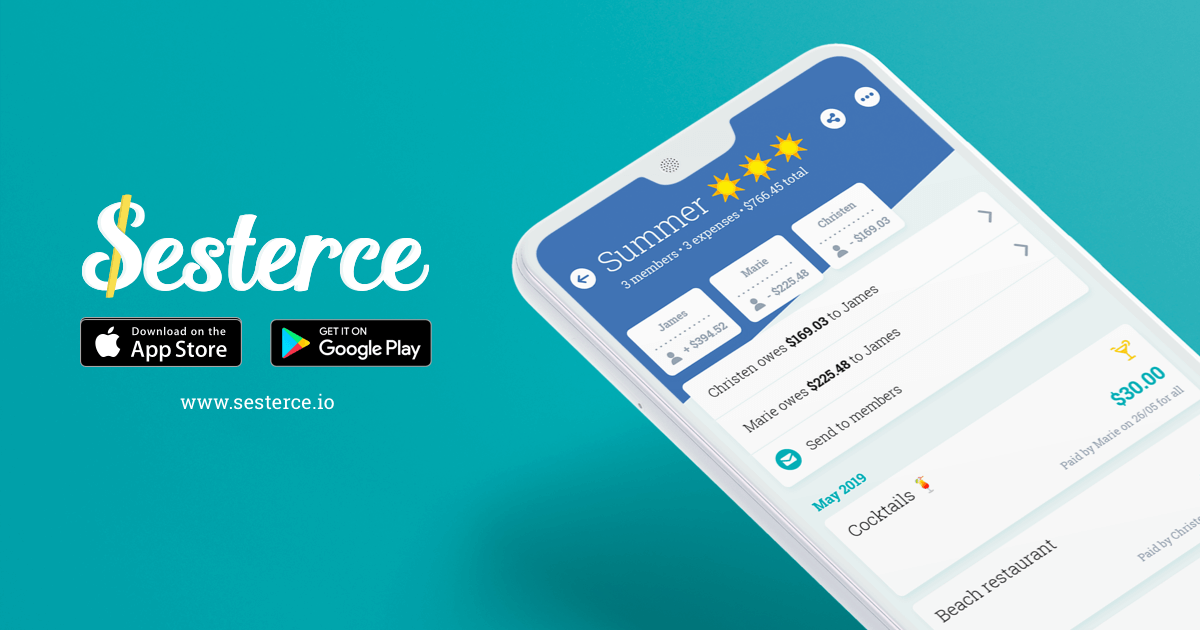
\includegraphics[width=50mm,scale=0.5]{img/logo-sesterce.png}}
            \caption{Sesterce}
            \label{fig:my_label}
        \end{figure}
        \begin{itemize}
            \item \textbf{Rating}: 4.7 stars (106 reviews) on Google Play Store
            \item \textbf{Downloads}: 5,000+ on Google Play Store
            \item \textbf{Features}:
                \begin{itemize}
                    \item Splitting expenses unevenly
                    \item Sort expenses by categories
                    \item View statistics by category and group member
                    \item Converting foreign currency
                    \item Export all data
                \end{itemize}
            \item \textbf{Differences}:
                \begin{itemize}
                    \item Nanuda does not have expense categories
                    \item No statistics
                    \item No conversion between currencies
                    \item Cannot export data
                \end{itemize}
        \end{itemize}
\end{enumerate}

\subsection{Task distribution}
\begin{table}[htbp]
\centering
\caption{Task Distribution}
\label{tab:task-distribution}
\begin{tabular}{|l|l|}
\hline
\textbf{Name}  & \textbf{Task}                    \\ \hline
Abia Putrama Herlianto & \begin{tabular}[c]{@{}l@{}}Balances Frontend, Backend,\\ Documentation\end{tabular} \\ \hline
Hugo Ravé      & Groups Frontend, Documentation   \\ \hline
Nadya Hartanto & Expenses Frontend, Documentation \\ \hline
\end{tabular}
\end{table}

\section{Specifications}
    \begin{enumerate}
        \item \textbf{Groups}
            \begin{figure}[H]
                \centerline{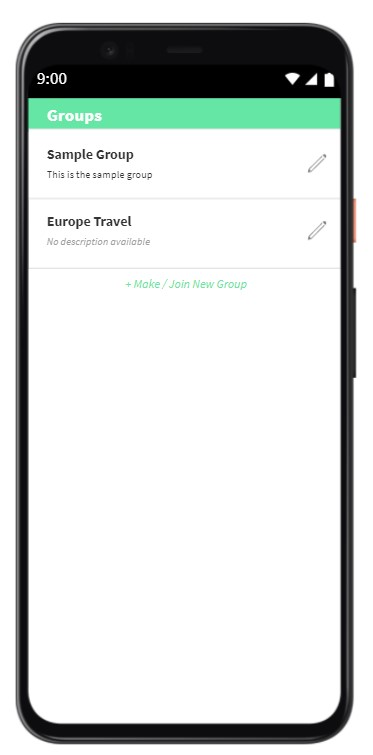
\includegraphics[scale=0.5]{img/ui/group-main.jpg}}
                \caption{Groups List Screen}
                \label{fig:groups-list-screen}
            \end{figure}
            \begin{figure}[H]
                \centerline{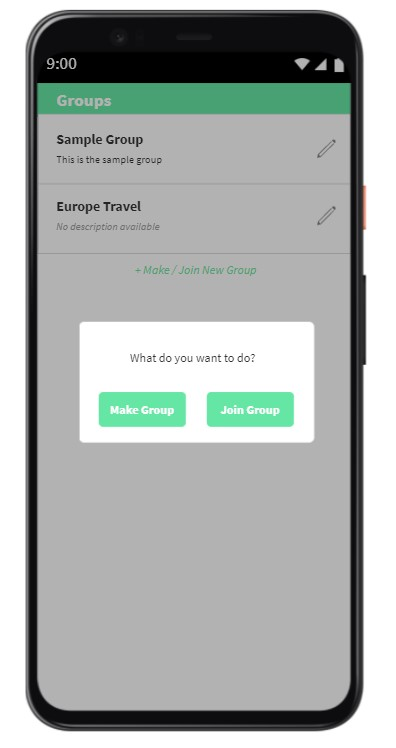
\includegraphics[scale=0.5]{img/ui/group-make-or-join.jpg}}
                \caption{Make New Group Screen}
                \label{fig:make-new-group-screen}
            \end{figure}
            \begin{figure}[H]
                \centerline{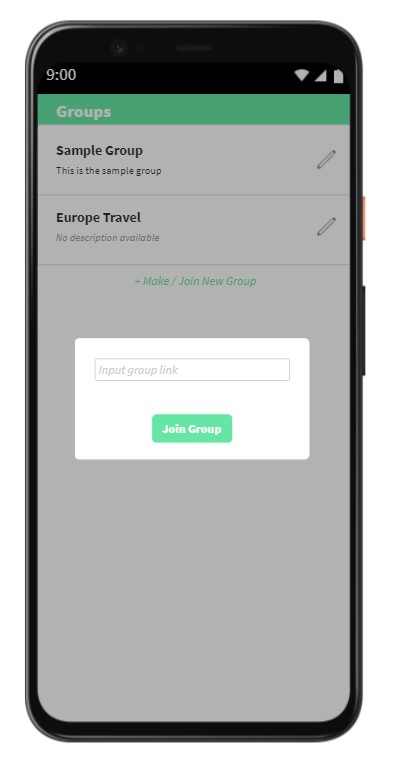
\includegraphics[scale=0.5]{img/ui/group-join.jpg}}
                \caption{Join Group Screen}
                \label{fig:join-group-screen}
            \end{figure}
            \begin{figure}[H]
                \centerline{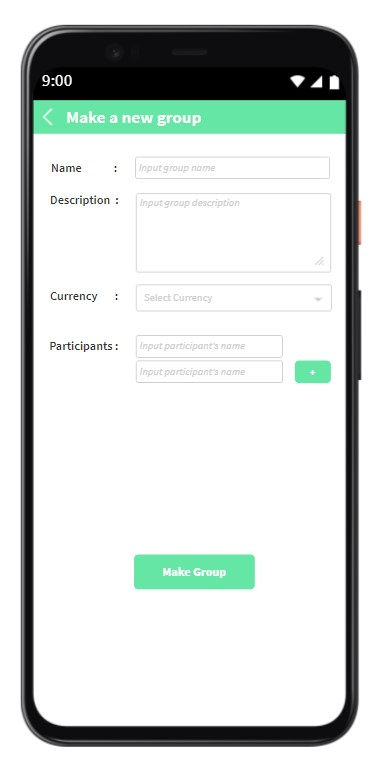
\includegraphics[scale=0.5]{img/ui/group-make.jpg}}
                \caption{Make Group Screen}
                \label{fig:make-group-screen}
            \end{figure}
            \begin{figure}[H]
                \centerline{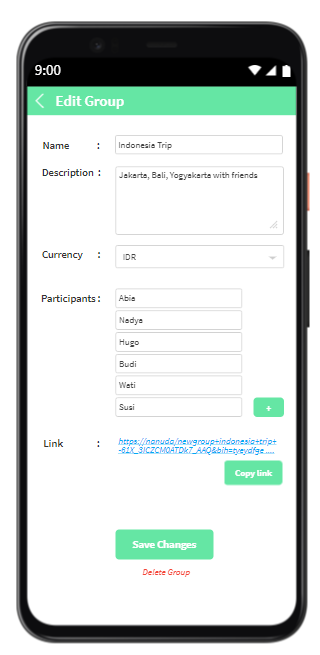
\includegraphics[scale=0.6]{img/ui/group-edit.png}}
                \caption{Edit Group Screen}
                \label{fig:edit-group-screen}
            \end{figure}
            \begin{enumerate}
                \item Groups List
                    \begin{enumerate}
                        \item The application should load the locally stored group ID data.
                        \item If it is the first time the application is opened, the application should create new locally stored group ID data. By default, a sample group with sample expenses should be made. After it is created, the new sample group should be uploaded to the server and added to the database.
                        \item The application should display a list of the existing groups.
                        \item For each group, its name and description are displayed.
                        \item The user should only be part of no more than 5 groups.
                    \end{enumerate}
                \item Enter Group
                    \begin{enumerate}
                        \item If the user clicks on a group, the application should move to the group's Expenses screen.
                    \end{enumerate}
                \item Add Group
                    \begin{enumerate}
                        \item If the user clicks the "Add Group" button, the application should display the "Add Group" pop up screen.
                        \item The application should display the "Make New Group" and "Join Group" buttons.
                        \item If the user is already part of 5 groups, the application should display an error informing the user that they have reached the maximum number of groups.
                    \end{enumerate}
                \item Make New Group
                    \begin{enumerate}
                        \item If the user clicks the "Make New Group" button, the application should display the "New Group" pop up screen.
                        \item The user should input the name of the new group, choose a currency to be used by the expenses in the group, and input the names of the participants of the new group.
                        \item The user should optionally be able to add a description to the new group.
                        \item The name of the new group should not be empty and should be no longer than 20 characters.
                        \item If there is a description, the description of the new group should be no longer than 50 characters.
                        \item The user should be able to choose one of at least three major currencies for the new group.
                        \item The user should be able to add participants' names by inputting the name and clicking the "Add" button.
                        \item The new group should have no more than 20 participants.
                        \item If the user clicks the "Create New Group" button, the application creates the new group and display a link to share to other users to join the group.
                        \item If the requirements for the new group have not been met, the "Create New Group" button should not be interactable.
                        \item If the user clicks the "Back" button, the application should move back to the groups list screen.
                    \end{enumerate}
                \item Join Group
                    \begin{enumerate}
                        \item If the user clicks the "Join Group" button, the application should display the "Join Group" pop up screen.
                        \item The user should input the link of the group they wish to join.
                        \item If the user clicks the "Join" button, the application sends a request to the server to find the group and download its information.
                        \item If the link has not been input or the link is invalid, the "Join" button should not be interactable.
                        \item If the user clicks the "Back" button, the application should move back to the groups list screen.
                    \end{enumerate}
                \item Edit Group
                    \begin{enumerate}
                        \item If the user clicks the "Edit Group" button, the application should display the "Edit Group" pop up screen.
                        \item The application should display the name, currency used by, and names of the participants of the group.
                        \item The user should be able to change the name, the description, the currency used by the expenses in the group, and the names of the participants of the group.
                        \item The name of the group should not be empty and should be no longer than 20 characters.
                        \item If there is a description, the description of the group should be no longer than 50 characters.
                        \item The user should be able to choose one of at least three major currencies for the new group.
                        \item The user should be able to add participants' names by inputting the name and clicking the "Add" button.
                        \item The group should have no more than 20 participants.
                        \item If the user clicks the "Save Changes" button, the application updates the group and moves back to the expenses list screen.
                        \item If the requirements for the group have not been met, the "Save Changes" button should not be interactable.
                        \item If the user clicks the "Back" button, the application should move back to the expenses list screen.
                    \end{enumerate}
                \item Sync Groups
                    \begin{enumerate}
                        \item If the user clicks the "Sync" button, the application should download the latest groups data from the server.
                    \end{enumerate}
                \item Delete Groups
                    \begin{enumerate}
                        \item If the user long-presses any group, the user should be able to select groups to be deleted.
                        \item If the user selects groups to be deleted, there should be a "Delete Groups" button to delete the groups.
                    \end{enumerate}
            \end{enumerate}
        \item \textbf{Expenses}
            \begin{figure}[H]
                \centerline{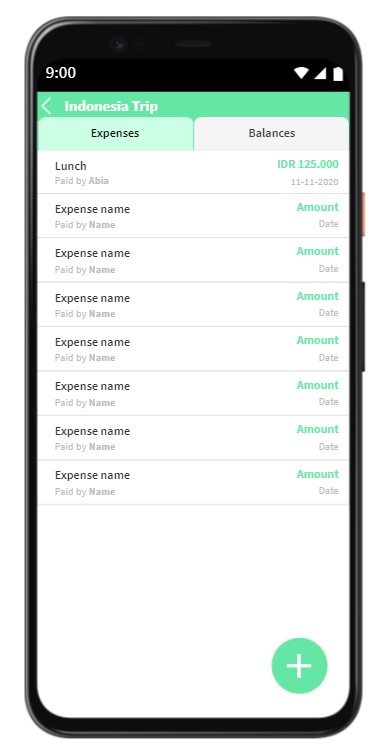
\includegraphics[scale=0.5]{img/ui/expenses-main.jpg}}
                \caption{Expenses Main Screen}
                \label{fig:expenses-main-screen}
            \end{figure}
            \begin{figure}[H]
                \centerline{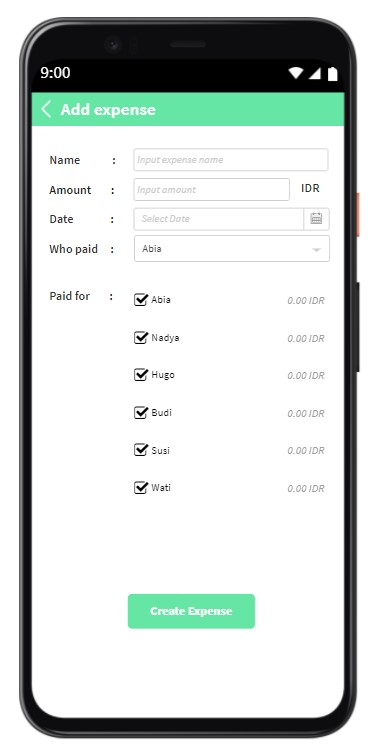
\includegraphics[scale=0.5]{img/ui/expenses-create.jpg}}
                \caption{Add Expense Screen}
                \label{fig:add-expense-screen}
            \end{figure}
            \begin{figure}[H]
                \centerline{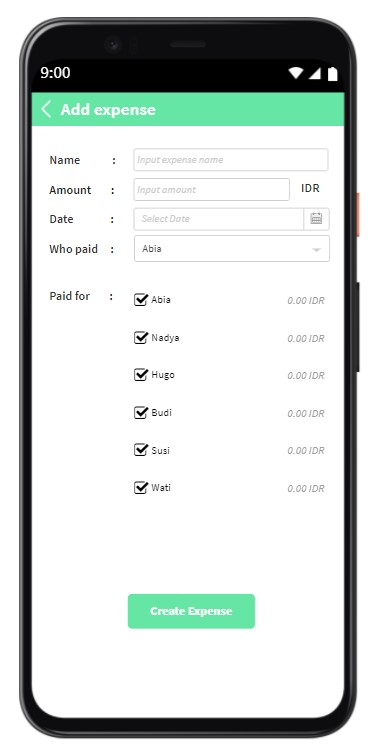
\includegraphics[scale=0.5]{img/ui/expenses-create.jpg}}
                \caption{Edit Expense Screen}
                \label{fig:edit-expense-screen}
            \end{figure}
            \begin{enumerate}
                \item Back Button
                    \begin{enumerate}
                        \item If the user clicks the "Back" button, the application should move back to the groups list screen.
                    \end{enumerate}
                \item Balances Button
                    \begin{enumerate}
                        \item If the user clicks the "Balances" button, the application should move to the balances screen.
                    \end{enumerate}
                \item Expenses List
                    \begin{enumerate}
                        \item The application should display a list of the existing expenses of the group.
                        \item For each expense, its name, amount, payer, and date should be displayed.
                        \item There should be no limit to the number of expenses in a group.
                    \end{enumerate}
                \item Enter Expense
                    \begin{enumerate}
                        \item If the user clicks on an expense, the application should display the details of the expense.
                        \item The application should display the name, amount, date, and payer of the expense. It should also display the participants who were paid for by this expense and how much each participant owes. It should also display the "Edit Expense" button.
                        \item If the user clicks the "Back" button, the application should move back to the expenses list screen.
                    \end{enumerate}
                \item Edit Expense
                    \begin{enumerate}
                        \item If the user clicks on the "Edit Expense" button, the application should display the "Edit Expense" pop up screen.
                        \item The application should display the name, amount, and date of the expense and choose the participant who pays and participants who are paid for.
                        \item The user should be able to change the name, amount, date of the expense, the participant who pays, and the participants who are paid for.
                        \item The name of the expense should not be empty and should be no longer than 20 characters.
                        \item The amount of the expense should not be empty.
                        \item The payer participant should not be empty and the user should choose a participant from the list of participants.
                        \item The application should display all the participants in the group under the "Paid For" label.
                        \item Next to each participant, there should be a checkbox so the user can choose whether the participant is paid for or not.
                        \item There should be a checkbox next to the "Paid For" label to choose all participants in the group.
                        \item Next to each participant whose checkbox is ticked, there should be the amount that will be owed by the participant. By default, the total amount expended should be divided equally between all paid for participants.
                        \item The user should optionally be able to change how much each participant will owe in the expense manually.
                        \item If the user edits how much each participant will owe in the expense manually, the total should be equal to the amount expended by the payer participant.
                        \item If the user clicks the "Save Changes" button, the application updates the expense and moves back to the expenses list screen.
                        \item If the requirements for the new expense have not been met, the "Save Changes" button should not be interactable.
                        \item If the user clicks the "Back" button, the application should move back to the expenses list screen.
                    \end{enumerate}
                \item Add Expense
                    \begin{enumerate}
                        \item If the user clicks the "Add Expense" button, the application should display the "New Expense" pop up screen.
                        \item The user should input the name, amount, and date of the expense and choose the participant who pays and the participants who are paid for.
                        \item The name of the expense should not be empty and should be no longer than 20 characters.
                        \item The amount of the expense should not be empty.
                        \item By default, the date of the expense should be the current date.
                        \item The payer participant should not be empty and the user should choose a participant from the list of participants.
                        \item The application should display all the participants in the group under the "Paid For" label.
                        \item Next to each participant, there should be a checkbox so the user can choose whether the participant is paid for or not.
                        \item There should be a checkbox next to the "Paid For" label to choose all participants in the group.
                        \item Next to each participant whose checkbox is ticked, there should be the amount that will be owed by the participant. By default, the total amount expended should be divided equally between all paid for participants.
                        \item The user should optionally be able to input how much each participant will owe in the expense manually.
                        \item If the user edits how much each participant will owe in the expense manually, the total should be equal to the amount expended by the payer participant.
                        \item If the user clicks the "Add Expense" button, the application creates the new expense and moves back to the expenses list screen.
                        \item If the requirements for the new expense have not been met, the "Add Expense" button should not be interactable.
                        \item If the user clicks the "Back" button, the application should move back to the expenses list screen.
                    \end{enumerate}
                \item Sync Expenses
                    \begin{enumerate}
                        \item If the user clicks the "Sync" button, the application should download the latest group expenses data from the server.
                    \end{enumerate}
            \end{enumerate}
        \item \textbf{Balances}
            \begin{figure}[htbp]
                \centerline{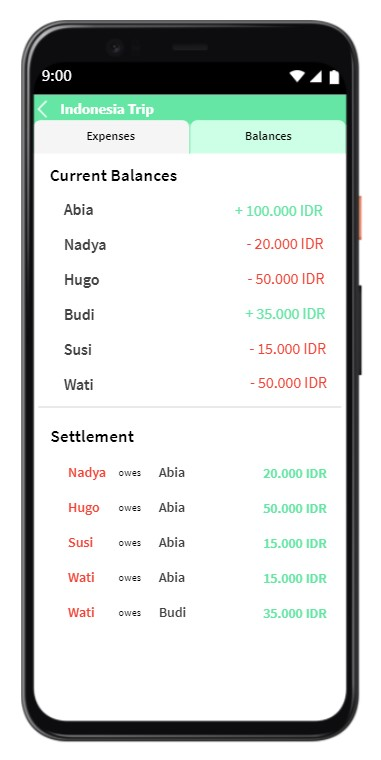
\includegraphics[scale=0.5]{img/ui/balances.jpg}}
                \caption{Balances Screen}
                \label{fig:balances-screen}
            \end{figure}
            \begin{enumerate}
                \item Back Button
                    \begin{enumerate}
                        \item If the user clicks the "Back" button, the application should move back to the groups list screen.
                    \end{enumerate}
                \item Expenses Button
                    \begin{enumerate}
                        \item If the user clicks the "Expenses" button, the application should move to the expenses screen.
                    \end{enumerate}
                \item Summary
                    \begin{enumerate}
                        \item The application should display the name of each participant in the group and how much they owe or are owed to.
                        \item If in total the participant owes more than they are owed, then the total amount they owe should be displayed with a red background.
                        \item If in total the participant is owed more than they owe, then the total amount they are owed should be displayed with a green background.
                    \end{enumerate}
                \item Balancing Details
                    \begin{enumerate}
                        \item The application should display how much each participant owes another participant in separate balances.
                    \end{enumerate}
            \end{enumerate}
    \end{enumerate}

\section{Architecture Design and Implementation}
\subsection{Overall architecture}
    \begin{figure}[H]
        \centerline{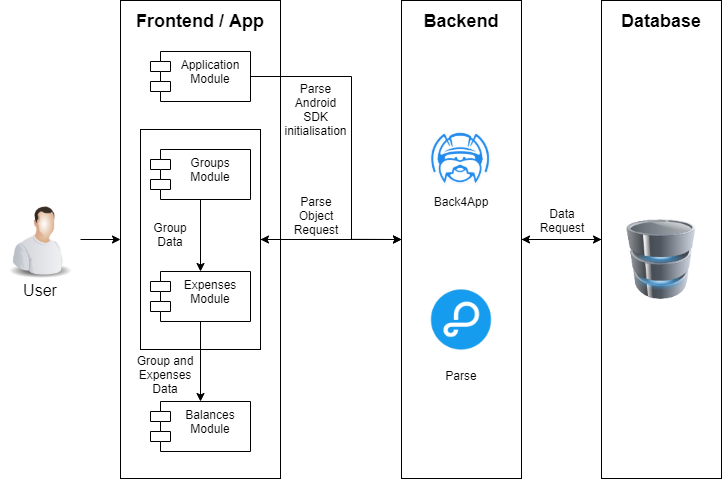
\includegraphics[scale=0.35]{img/overall_architecture.png}}
        \caption{Overall Architecture}
        \label{fig:overall-architecture}
    \end{figure}

The Nanuda Android application is divided into four separate modules.

The first part is the "Application" module which is responsible for setting up and starting the application. The "Application" module does this by initialising the application, splash screen, and everything required to connect to the backend. Nanuda uses the low-code back4app open source Backend as a Service provider for its backend, which means Nanuda does not have a separate backend module. Instead, the "Application" module is responsible for connecting and allowing itself as well as other modules to connect to the backend.

The second part is the "Groups" module which is responsible for displaying, adding, joining, editing, and deleting groups. It interacts with the backend to get, add, edit, and remove group data.

The third part is the "Expenses" module which is responsible for displaying, adding, editing, and deleting expenses. It interacts with the backend to get, add, edit, and remove expense data.

The fourth part is the "Balances" module which is responsible for calculating and displaying the summaries of how much each user owes or is owed in total and how users can settle them.

These four modules interact with each other as well as the backend in order for the application to function.

\subsection{Directory organization}
The organisation of Nanuda's directories follows the organisation of an Android Studio project. Generally, the organisation of the Java packages in the Android Studio project closely follows the overall architecture which splits the application into four modules. In addition, there is a separate directory for files related to the documentation of the project.

\begin{table}[H]
\centering
\caption{Directory Organization}
\label{tab:directory-organization-1}
\begin{tabular}{|l|l|l|}
\hline
\textbf{Directory} &
  \textbf{File Name} &
  \textbf{\begin{tabular}[c]{@{}l@{}}Module \\ Name\end{tabular}} \\ \hline
\begin{tabular}[c]{@{}l@{}}\textbackslash{}app\textbackslash{}src\textbackslash{}main\\ \textbackslash{}java\textbackslash{}com\\ \textbackslash{}teammoney\\ \textbackslash{}nanuda\end{tabular} &
  \begin{tabular}[c]{@{}l@{}}Nanuda.java\\ SplashScreenActivity.java\end{tabular} &
  Application \\ \hline
\begin{tabular}[c]{@{}l@{}}\textbackslash{}app\textbackslash{}src\textbackslash{}main\\ \textbackslash{}java\textbackslash{}com\\ \textbackslash{}teammoney\\ \textbackslash{}nanuda\textbackslash{}objects\end{tabular} &
  \begin{tabular}[c]{@{}l@{}}Expense.java\\ Group.java\end{tabular} &
  Application \\ \hline
\begin{tabular}[c]{@{}l@{}}\textbackslash{}app\textbackslash{}src\textbackslash{}main\\ \textbackslash{}java\textbackslash{}com\\ \textbackslash{}teammoney\\ \textbackslash{}nanuda\textbackslash{}expense\end{tabular} &
  \begin{tabular}[c]{@{}l@{}}ExpensesListActivity.java\\ ExpenseAdapter.java\\ MakeExpenseActivity.java\\ EditExpenseActivity.java\end{tabular} &
  Expenses \\ \hline
\begin{tabular}[c]{@{}l@{}}\textbackslash{}app\textbackslash{}src\textbackslash{}main\\ \textbackslash{}java\textbackslash{}com\\ \textbackslash{}teammoney\\ \textbackslash{}nanuda\textbackslash{}group\end{tabular} &
  \begin{tabular}[c]{@{}l@{}}GroupsListActivity.java\\ MakeGroupActivity.java\\ EditGroupActivity.java\end{tabular} &
  Groups \\ \hline
\begin{tabular}[c]{@{}l@{}}\textbackslash{}app\textbackslash{}src\textbackslash{}main\\ \textbackslash{}java\textbackslash{}com\\ \textbackslash{}teammoney\\ \textbackslash{}nanuda\textbackslash{}balances\end{tabular} &
  \begin{tabular}[c]{@{}l@{}}BalancesActivity.java\\ BalancesAdapter.java\end{tabular} &
  Balances \\ \hline
\textbackslash{}docs &
  \begin{tabular}[c]{@{}l@{}}documentation.pdf\\ documentation.tex\end{tabular} &
  \begin{tabular}[c]{@{}l@{}}Documen\\ -tation\end{tabular} \\ \hline
\begin{tabular}[c]{@{}l@{}}\textbackslash{}app\textbackslash{}src\textbackslash{}main\\ \textbackslash{}res\textbackslash{}drawable\end{tabular} &
  \begin{tabular}[c]{@{}l@{}}ic\_baseline\_arrow\_back\_ios\_24.xml\\ ic\_launcher\_background.xml\\ splash\_screen\_background.xml\end{tabular} &
  \begin{tabular}[c]{@{}l@{}}Application\\ Groups\\ Expenses\\ Balances\end{tabular} \\ \hline
\begin{tabular}[c]{@{}l@{}}\textbackslash{}app\textbackslash{}src\textbackslash{}main\\ \textbackslash{}res\textbackslash{}layout\end{tabular} &
  \begin{tabular}[c]{@{}l@{}}activity\_edit\_expense.xml\\ activity\_edit\_group.xml\\ activity\_expenses\_lists.xml\\ activity\_groups\_list.xml\\ activity\_make\_expense.xml\\ activity\_make\_group.xml\\ activity\_splash\_screen.xml\\ expenses\_list\_item.xml\\ group\_toolbar.xml\\ join\_popup.xml\\ make\_new\_group\_toolbar.xml\end{tabular} &
  \begin{tabular}[c]{@{}l@{}}Application\\ Groups\\ Expenses\\ Balances\end{tabular} \\ \hline
\begin{tabular}[c]{@{}l@{}}\textbackslash{}app\textbackslash{}src\textbackslash{}main\\ \textbackslash{}res\textbackslash{}menu\end{tabular} &
  join\_group\_menu.xml &
  Groups \\ \hline
\begin{tabular}[c]{@{}l@{}}\textbackslash{}app\textbackslash{}src\textbackslash{}main\\ \textbackslash{}res\textbackslash{}values\end{tabular} &
  \begin{tabular}[c]{@{}l@{}}colors.xml\\ dimens.xml\\ ids.xml\\ strings.xml\\ themes.xml\end{tabular} &
  \begin{tabular}[c]{@{}l@{}}Application\\ Groups\\ Expenses\\ Balances\end{tabular} \\ \hline
\end{tabular}
\end{table}

\subsection{Module 1: Application}
    \begin{figure}[H]
        \centerline{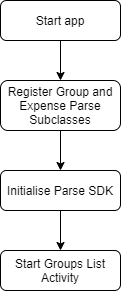
\includegraphics[scale=0.3]{img/flowcharts/flowchart-module-application.png}}
        \caption{Application Module Flowchart}
        \label{fig:application-module-flowchart}
    \end{figure}
\begin{itemize}
    \item Purpose \\ The Application module is responsible for initialising the app and its connection with the backend as well as defining information required by the app to function properly.
    \item Functionality \\ It starts the app, connects it with the backend, and defines the Parse Objects to be used by the Android Parse SDK by the application.
    \item Location of Source Code
        \begin{itemize}
            \item nanuda\textbackslash{}app\textbackslash{}src\textbackslash{}main\textbackslash{}java\textbackslash{}com\textbackslash{}teammoney\textbackslash{}nanuda
            \item nanuda\textbackslash{}app\textbackslash{}src\textbackslash{}main\textbackslash{}java\textbackslash{}com\textbackslash{}teammoney\textbackslash{}nanuda\textbackslash{} objects
        \end{itemize}
    \item Class Components
        \begin{itemize}
            \item Nanuda.java \\ Registers the Parse Object subclasses "Group" and "Expense" as required by the SDK and initialises the Parse SDK with the app's application ID, client key, and connects it to the backend at back4app.
            \item SplashScreenActivity.java \\ Sends an intent from the Splash Screen to the Groups List to start the Groups List Activity.
            \item Group.java \\ Defines the Group Parse Object subclass as the local Android implementation of the Group table in the backend.
            \item Expense.java \\ Defines the Expense Parse Object subclass as the local Android implementation of the Expense table in the backend.
        \end{itemize}
    \item Where It's Taken From \\ We developed the module ourselves using resources from Back4App and Parse Platform's documentation at https://www.back4app.com/docs and https://docs.parseplatform.org/android/guide respectively.
    \item How/Why We Use It \\ The Groups module was made because it is one of the three main features of Nanuda. To make it into its own module with its own functionalities and required data is intuitive and makes the development simpler.
\end{itemize}

\subsection{Module 2: Groups}
    \begin{figure}[H]
        \centerline{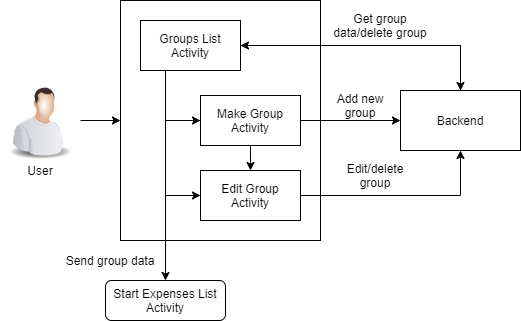
\includegraphics[scale=0.4]{img/flowcharts/flowchart-module-groups.png}}
        \caption{Groups Module}
        \label{fig:groups-module-flowchart}
    \end{figure}
\begin{itemize}
    \item Purpose \\ The Groups module is responsible for displaying, making, joining, editing, and deleting groups.
    \item Functionality \\ It gets a list of groups the user has joined from the locally-stored file groups.txt and sends a query to the backend to get the groups' data. It displays all these groups. It  also allows the user to make a new group and join, edit, and delete existing groups.
    \item Location of Source Code \\ nanuda\textbackslash{}app\textbackslash{}src\textbackslash{}main\textbackslash{}java\textbackslash{}com\textbackslash{}teammoney\textbackslash{}nanuda\textbackslash{}group
    \item Class Components
        \begin{itemize}
            \item GroupsListActivity.java \\ Reads the group IDs of the groups the user has joined from the locally-stored groups.txt file and sends a query to the backend to get the groups' data. Using the group data, it creates a Recycler View with each group as a list item. For each list item, it sets up an OnClickListener so that if a user clicks a group, it will send an intent to the Expenses List to start the Expenses List activity. It also sets up the the "Make/Join Group" button, the "Make/Join Group" popup, and the "Join Group" popup. Also sets up the functionality for group list items so that when they are long-pressed, they show a delete option.
            \item MakeGroupActivity.java \\ Sets up the make group form and sends a request to the backend to create a group using the provided information.
            \item EditGroupActivity.java \\ Sets up the edit group form with the group's existing data and sends a request to the backend to edit the group using the provided information.
        \end{itemize}
    \item Where It's Taken From \\ We developed the module ourselves using resources from Back4App and Parse Platform's documentation at https://www.back4app.com/docs and https://docs.parseplatform.org/android/guide respectively.
    \item How/Why We Use It \\ The Expenses module was made because it is one of the three main features of Nanuda. To make it into its own module with its own functionalities and required data is intuitive and makes the development simpler.
\end{itemize}

\subsection{Module 3: Expenses}
    \begin{figure}[H]
        \centerline{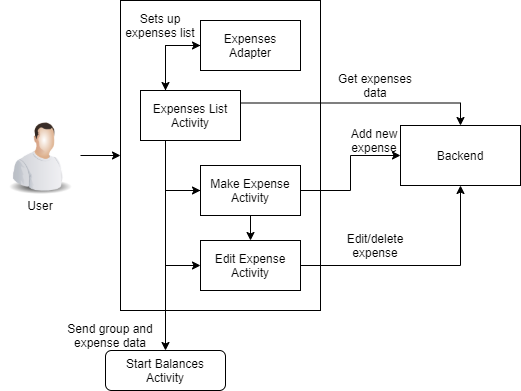
\includegraphics[scale=0.3]{img/flowcharts/flowchart-module-expenses.png}}
        \caption{Expenses Module}
        \label{fig:expenses-module-flowchart}
    \end{figure}
\begin{itemize}
    \item Purpose \\ The Expenses module is responsible for displaying, making, editing, and deleting expenses.
    \item Functionality \\ It receives the Group data, queries for all the expenses associated with that group, and displays them. It also allows the user to add new expenses and edit and delete existing ones.
    \item Location of Source Code \\ nanuda\textbackslash{}app\textbackslash{}src\textbackslash{}main\textbackslash{}java\textbackslash{}com\textbackslash{}teammoney\textbackslash{}nanuda\textbackslash{}expense
    \item Class Components
        \begin{itemize}
            \item ExpensesListActivity.java \\ Sets the "Expenses" tab as the selected tab, adds an OnTabSelectedListener to the "Balances" tab so that when the user selects it it will send an intent to the Balances and start the Balances Activity, gets the group data and queries the backend for all expenses associated with that group and passes that data to the Expenses Adapter to make it into a Recycler View.
            \item ExpensesAdapter.java \\ Adapts the expenses list provided by ExpensesListActivity.java into Recycler View form.
            \item MakeExpenseActivity.java \\ Sets up the make expense form and sends a request to the backend to create an expense using the provided information.
            \item EditExpenseActivity.java \\ Sets up the edit expenses form with the expense's existing data and sends a request to the backend to edit the expense using the provided information.
        \end{itemize}
\end{itemize}

\subsection{Module 4: Balances}
    \begin{figure}[H]
        \centerline{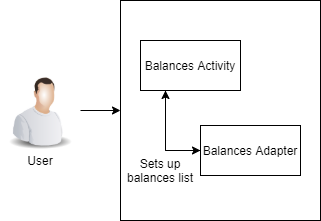
\includegraphics[scale=0.5]{img/flowcharts/flowchart-module-balances.png}}
        \caption{Balances Module}
        \label{fig:balances-module-flowchart}
    \end{figure}
\begin{itemize}
    \item Purpose \\ The Balances module is responsible for calculating and displaying the summary of how much each user owes or is owed and how to settle them.
    \item Functionality \\ It receives the Group and Expenses data, counts the summary for each user, calculates how participants in debt should pay the other participants that are indebted to.
    \item Location of Source Code \\ nanuda\textbackslash{}app\textbackslash{}src\textbackslash{}main\textbackslash{}java\textbackslash{}com\textbackslash{}teammoney\textbackslash{}nanuda\textbackslash{}balances
    \item Class Components
        \begin{itemize}
            \item BalancesActivity.java \\ Sets the "Balances" tab as the selected tab, adds an OnTabSelectedListener to the "Expenses" tab so that when the user selects it it will send an intent to the Expenses List and start the Expenses List Activity, calculates the total of how much each user owes or is owed, how to settle them, and passes that data to the Recycler View adapter. To calculate the total of how much each user owes or is owed, the algorithm goes through each Expense and adds it to or subtracts it from the payer's total. To calculate how to settle it, the algorithm sorts the users who owe and the users who are owed to in descending order separately. Then starting from the user who is owed the most, 
            the algorithm goes through the users who owe and has them pay the amount owed. It continues this until the entire amount owed is accounted for.
            \item BalancesAdapter.java \\
            Adapts the summary list and details list provided by BalancesActivity.java into Recycler View form. In order to optimise the code, both lists as well as their headers are part of a single long RecyclerView. First, the header of the summary list is entered into the Recycler View, followed by the summary list items, the header of the details list, and finally the details list items.
        \end{itemize}
    \item Where It's Taken From \\ We developed the module ourselves using resources from Back4App and Parse Platform's documentation at https://www.back4app.com/docs and https://docs.parseplatform.org/android/guide respectively.
    \item How/Why We Use It \\ The Balances module was made because it is one of the three main features of Nanuda. To make it into its own module with its own functionalities and required data is intuitive and makes the development simpler.
\end{itemize}

\end{document}
